

\chapter{绪论}

\section{研究背景及意义}
% \subsection{二级标题}
显示技术是人类感知客观世界的重要媒介，在推进社会进步与科技创新方面具有不可替代的战略价值，现已成为驱动信息化社会发展的关键技术引擎之一。

\begin{figure}[htbp]
  \centering
  % 第一张子图
  \begin{minipage}{0.49\textwidth}
    \centering
    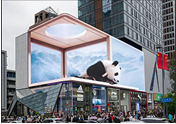
\includegraphics[width=0.9\linewidth, height=4cm]{resources/1p/1-1a.png}
    
    \centering\small(a)
    \label{fig:1-1a}
  \end{minipage}
  \hfill
  % 第二张子图
  \begin{minipage}{0.49\textwidth}
    \centering
    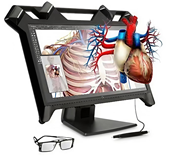
\includegraphics[width=0.9\linewidth, height=4cm]{resources/1p/1-1b.png}
    
    \centering\small(b)
    \label{fig:1-1b}
  \end{minipage}

  \vspace{0.5cm}

  % 第三张子图
  \begin{minipage}{0.49\textwidth}
    \centering
    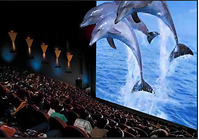
\includegraphics[width=0.9\linewidth, height=4cm]{resources/1p/1-1c.png}
    
    \centering\small(c) 
    \label{fig:1-1c}
  \end{minipage}
  \hfill
  % 第四张子图
  \begin{minipage}{0.49\textwidth}
    \centering
    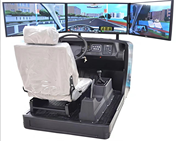
\includegraphics[width=0.9\linewidth, height=4cm]{resources/1p/1-1d.png}
    
    \centering\small(d) 
    \label{fig:1-1d}
  \end{minipage}

  \caption{三维显示技术的典型应用场景 (a)3D广告 (b)三维医疗 (c)3D电影 (d)三维模拟驾驶}
  \label{fig:1-1}
\end{figure}

  



当前，日常生活中主流的显示方式仍以二维平面显示为主导。这种显示模式无法为观察者提供有效的深度感知信息，仅能呈现三维场景的单一视角投影，导致深度维度信息的缺失，限制了人们对客观事物的全面认知。在工业造型设计、户外广告传媒、医学教育培训以及军事仿真作战等诸多应用领域，三维显示技术\cite{Hua2022}展现出广阔的发展前景。能体现出更真实\cite{李涵宇2025}的效果，作为下一代显示技术的核心演进方向，三维显示正在加速向生产生活各领域渗透\cite{Li2023}。

从工业制造到商业推广，如图所示该技术体现出显著的应用价值：在商业广告领域，如图~\ref{fig:1-1}(a)所示，三维显示技术重构了广告传播的呈现形式。相较于传统二维广告的平面化表达，三维广告能够精准还原产品的立体结构、细节纹理及空间形态，借助光影渲染增强视觉层次感\cite{Wang2021a}，既能够让受众直观感知产品核心优势，又能通过沉浸式视觉体验吸引注意力，有效提升广告传播效率，助力企业强化品牌认知，进一步推动产品转化率的提升，成为当下商业营销升级的重要突破口。在三维医疗领域，如图~\ref{fig:1-1}(b)所示，三维显示技术为医学诊疗与研究提供了有力支撑\cite{Chen2022}。该技术可将医学影像数据转化为逼真的三维立体模型，精准还原人体器官、组织的空间位置关系、形态结构及病变区域\cite{Zhang2020}，帮助医师更清晰地把握病灶特征，不仅大幅缩短术前规划时间、提升手术精准度，还能为医学教学、病例研讨提供直观的可视化载体，助力医学人才培养和诊疗技术的革新。在三维电影领域，如图~\ref{fig:1-1}(c)所示，三维显示技术推动了影视产业的业态升级\cite{Hu2022}。通过模拟人眼双目视觉原理\cite{Yang2021}，三维电影能够构建出立体逼真的影视场景，让观众突破屏幕局限，获得“身临其境”的观影体验，既丰富了影视内容的呈现形式，又增强了作品的视觉感染力，推动影视产业从二维向三维转型，带动了影视制作、放映等相关产业链的协同发展。在三维模拟驾驶领域，如图~\ref{fig:1-1}(d)所示，三维显示技术成为驾驶培训与研发的核心支撑\cite{Liu2022}。该技术可精准构建复杂的道路环境、交通场景及车辆运行状态，还原不同天气、路况下的驾驶场景\cite{Zhang2022a}，既能够为驾驶学习者提供安全、高效的模拟训练环境，降低实操培训风险和成本，又能为车辆研发、交通管控系统优化提供可视化模拟平台，助力提升驾驶安全水平和交通管理效能。

随着显示技术的进步，3D显示技术有了很大的进步，目前能够商用的显示技术主要分为需要佩戴外部设备的3D显示\cite{Sun2021}和不需要佩戴外部设备的裸眼3D显示技术，如图\ref{fig:1-2}所示：

\begin{figure}[htbp]
  \centering
  % 第一张子图（上方）
  \begin{minipage}{0.8\textwidth}  % 宽度保持和原格式一致，也可改为0.8\textwidth让图更宽
    \centering
    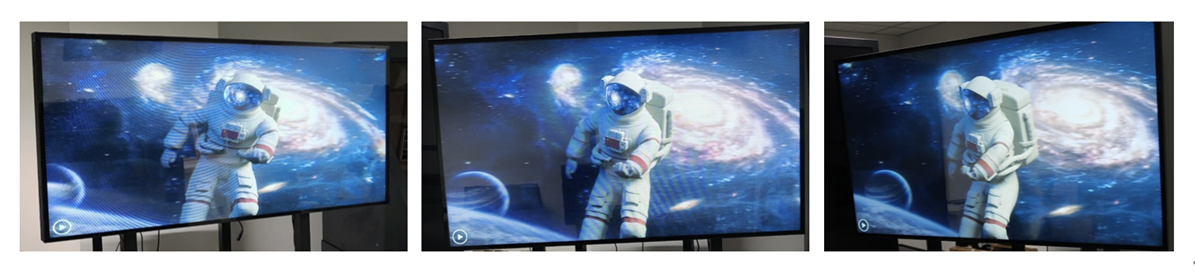
\includegraphics[width=0.9\linewidth, height=3cm]{resources/1p/1-2a.png}
    
    \centering\small(a)
    \label{fig:1-2a}
  \end{minipage}

  \vspace{0.5cm}  % 上下子图的间距，比原0.5cm稍大更美观，可按需调整

  % 第二张子图（下方）
  \begin{minipage}{0.8\textwidth}
    \centering
    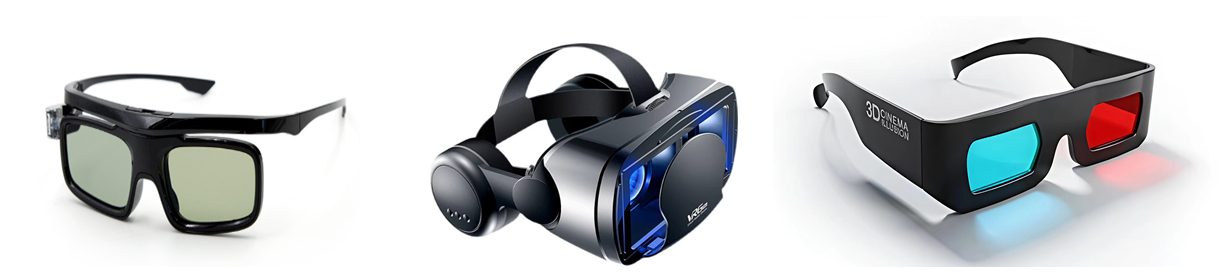
\includegraphics[width=0.9\linewidth, height=3cm]{resources/1p/1-2b.png}
    
    \centering\small(b)
    \label{fig:1-2b}
  \end{minipage}

  % 大图标题：仅保留两张子图的说明
  \caption{ (a)裸眼显示 (b)助眼显示}
  \label{fig:1-2}
\end{figure}

裸眼3D显示与传统需要佩戴专用辅助设备的三维显示方式存在显著区别，裸眼3D显示技术在不需要任何辅助设备的前提下，即可直接向观看者呈现立体视觉效果。相较于传统佩戴式三维显示，裸眼三维显示不仅彻底摆脱了辅助设备带来的佩戴束缚，避免了长时间佩戴设备产生的眩晕感、不适感，大幅提升了观看的便捷性和舒适度；还打破了佩戴设备对观看人数、观看场景的限制，无需观看者额外携带或佩戴相关器材，可支持多人同时观看，适配更多公共场景和私人场景，降低了三维显示技术的应用门槛，进一步拓宽了其应用范围，为三维显示技术的普及和多领域深度应用奠定了坚实基础。

在真实物理空间中，物体表面的明暗变化主要由入射光方向、强度以及材质反射特性共同决定。合理的光照与阴影分布不仅能够揭示物体的几何结构，还能够强化空间层次与体积感，使观察者在视觉上更容易感知深度关系与空间位置。

光线对人像立体感的塑造效果差异显著。在有合理光照的人像中，光线在面部形成自然的明暗过渡，突出额头、鼻梁、颧骨等高光区域，并在眼窝、鼻底、下颌下方形成柔和的过渡阴影，清晰还原了面部骨骼结构与肌肉起伏，使人像轮廓饱满、层次分明，呈现出强烈的立体感与真实的空间质感；而在无明显光照的对比图像中，面部明暗变化微弱，缺乏光影对比，整体显得扁平单调，难以体现出人脸应有的三维结构与体积感，如图 \ref {fig:1-3} 所示。

\begin{figure}[htbp]
  \centering
  % 第一张子图（左侧）
  \begin{minipage}{0.48\textwidth}  % 宽度减半，为左右排列留出空间
    \centering
    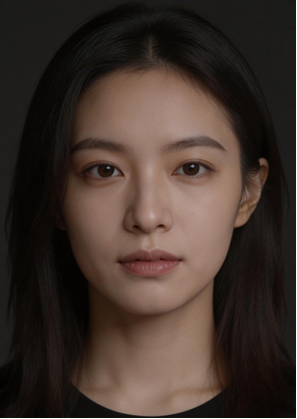
\includegraphics[width=0.9\linewidth, height=8cm]{resources/1p/1-3a.png}
    
    \centering\small(a) 
    \label{fig:1-2a}
  \end{minipage}
  \hfill  % 关键：添加水平间距，让两张图左右分开
  % 第二张子图（右侧）
  \begin{minipage}{0.48\textwidth}
    \centering
    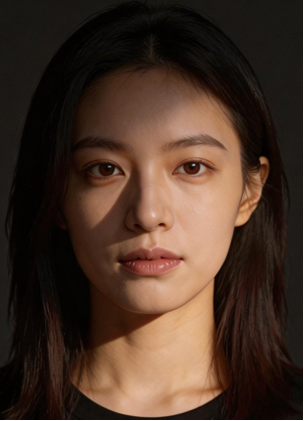
\includegraphics[width=0.9\linewidth, height=8cm]{resources/1p/1-3b.png}
    
    \centering\small(b) 
    \label{fig:1-2b}
  \end{minipage}

  % 大图标题：保持不变
  \caption{ (a)无光照的人像 (b)有光照的人像}
  \label{fig:1-3}
\end{figure}

由此可见，合适的光线与阴影分布是凸显人像立体感、还原真实空间形态的关键因素。这一规律同样适用于三维光场显示系统。与传统二维显示不同，三维光场显示通过重建多视角光线分布来还原真实场景中的光线传播状态，而光照信息正是其中决定真实感与沉浸感的核心要素之一。若光照方向错误或强度分布不合理，即使几何结构准确，也会导致画面失真、层次模糊，进而削弱立体感与空间可信度。

在静态三维光场人像显示中，光照的作用首先体现在对面部结构与细节纹理的塑造上。面部的高光区域、阴影过渡以及环境光的柔化效果能够清晰勾勒五官轮廓，突出鼻梁、颧骨与下颌线等关键结构，从而增强视觉立体度与真实度。适当的侧光或顶光可以有效提升人物的空间分离度，使主体从背景中自然凸显出来。同时，通过对光照颜色与强度的精确编辑，还能够传达情绪氛围与艺术风格，实现技术真实与视觉美感之间的平衡。因此，在静态光场人像重建与显示过程中，光照编辑不仅是一种后期增强手段，更是一种直接影响三维感知质量的基础环节。

而在动态三维光场人脸视频显示中，光照的重要性进一步放大。与静态场景相比，动态视频不仅包含空间维度变化，还叠加了时间维度上的连续运动信息。此时，光照的一致性、时序稳定性以及物理合理性将直接影响观看者的连续视觉体验。如果相邻帧之间光照分布突变或阴影跳变，将产生明显的闪烁与违和感，破坏沉浸效果，甚至引发视觉疲劳。因此，动态光照编辑需要在保证物理一致性的前提下，实现跨帧光照平滑过渡与多视角协同一致，以维持整体场景的真实连续性。

综上所述，无论是静态三维光场人像显示还是动态三维光场人像视频显示，光照始终是构建立体真实感与空间可信度的关键因素。光照编辑不仅影响单帧画面的明暗层次与几何表现，还决定了跨时间维度的视觉连贯性与沉浸体验质量。在三维光场显示研究与系统实现中，光照编辑是提升整体显示效果与用户感知质量的必要路径。

然而，现有三维光场人像光照编辑方法在实际应用中仍面临诸多挑战，比如采集设备繁琐，系统成本高昂，或者是编辑结果缺乏真实感，多视角一致性不足等问题。基于此，本课题聚焦三维光场显示中的人脸光照编辑，开展深入研究与创新，旨在为三维光场显示提供、高质量的内容支撑。


\section{研究现状}
\subsection{三维光场静态人像光照编辑的研究现状}
近年来，三维光场技术取得显著进步，三维光场显示可以提供理想的立体视觉体验，观者在其中观看三维场景就像它们存在于真实空间一样。它能够提升虚拟现实等领域的用户体验，对于数字媒体和人机交互的发展起到重要影响\cite{Bruno2010,Ho2020,Yang2013}。真实空间中，物体的明暗分布取决于光照，光照与阴影可以凸显画面的深度\cite{陈嘉琪2018,Todd2025}。而在三维光场显示中，光照同样是增加 3D 显示真实感和空间感的重要因素，通过编辑光照，可以大大提升立体显示效果。而合理准确的光照对于三维光场的显示效果起到非常关键的作用，光照编辑是三维光场中用于调整三维光场显示效果的常用方法。目前，对于三维光场人像光照编辑有两种方式。分别是多视图同时编辑方法和基于光照条件的密集视点采集方法\cite{Yang2023}。
多视图同时编辑方法，本质是对单张人像进行编辑，如图\ref{fig:single}所示,通过对多张视差图同时进行光照编辑的方法，从而达到对三维光场人像的编辑。

\begin{figure}[htbp]
  \centering
  %\vspace{1 cm} % 使用该指令调整上下间距
  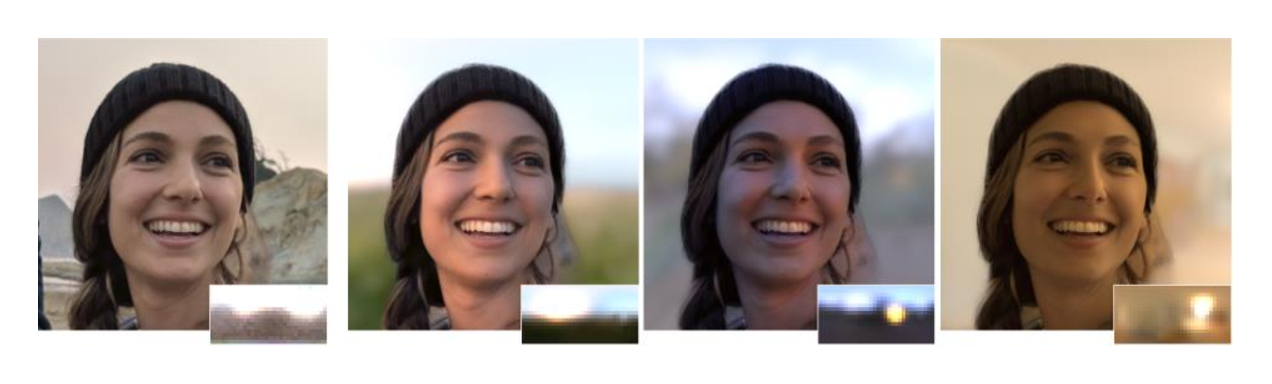
\includegraphics[width=0.7\textwidth,height=3cm]{resources/1p/1-single.pdf}
  % \bicaption{单张人像重光照}{English Caption} % 使用中英文标题
  \caption{单张人像重光照} % 只使用中文标题
  \label{fig:single}
  %\vspace{1 cm} % 使用该指令调整上下间距
\end{figure}

基于Chen提出的局部约束的全局优化实现光照编辑方法\cite{Chen2010}，是先构建局部光照约束，再通过全局优化算法调整整体光照效果，从而灵活改变人脸受光强度、方向等，实现自然的光照重新渲染。Liang提出的自适应编辑传播的人脸图像光照编辑\cite{梁凌宇2015}，通过融合参考人脸与目标背景、提取光照信息后，经自适应编辑传播生成光照模板并与目标人脸融合，实现光照编辑。Adobe Research 提出的SynthLight模型，将图像重光照建模转换成基于环境光照条件的像素重渲染问题，利用 Stable Diffusion\cite{Rombach2022}扩展的模型，并采用多任务训练策略和推理时的分类器自由引导机制，实现对 2D 人像的重光照\cite{Chaturvedi2025}。基于Xu等人提出了一种人像重光照系统，将标准手机相机拍摄的单张人像 RGB 图像作为输入，可生成在任意给定环境光照下的重光照图像，仅使用单个 RGB 肖像图和新的目标高动态范围照明环境作为输入就能实现更换背景重打光\cite{Sun2019}。基于商图像的多任务人脸光照编辑方法是通过预处理、商图像特征提取、特征扩散以及图像融合等步骤，在一个技术框架内同时实现人脸的光照迁移和重光照。IC-Light \cite{Zhang2025}方法基于光传输独立性原理，借助扩散模型\cite{Nichol2021,Rombach2022,Wang2024}和多层感知器，在训练中施加一致光传输约束，从而实现 2D 人像重光照。然而，三维光场内容由多视图构成，不同视图间的光照信息相互关联，当单独处理某一单张视图的光照时，会使多视图之间的光照一致性得不到保证,进而削弱三维光场的真实感与连贯性。

基于光照条件的密集视点采集方法如下，基于Paul 提出的light stage方法\cite{Debevec1999}，通过环形阵列光源依次点亮并同步拍摄，可采集人脸在不同光照条件下的高分辨率反射特性数据，可捕获数百乃至数千种不同光照方向、强度和颜色的面部反射数据，形成包含漫反射、镜面反射、次表面散射等多重物理特性的反射场\cite{Hanrahan1993}，结合 3D 几何模型实现后期任意角度的重光照渲染。上海科技大学 MARS 实验室提出的基于OLAT的采集方法，通过搭建由 114 个 LED 光源和一台 1000fps 的 4K 超高速摄像机组成的穹顶光场，在动态光照环境下可以达到更稳定人相重光照的视觉效果\cite{Zhang2021}。Shen提出的基于辐射场生成高质量光场人像的方法\cite{Shen2024}，能从任意视角和光照生成人像图像，通过分离场景几何和光照信息，生成高质量光场人像重光照结果，但是需要带偏振片的拍摄设备\cite{沈圣2025}。谷歌提出的人像照明技术，使用安装在球面内的 331 个 LED 灯进行拍摄，每次打开一个 LED 灯记录一个独立的光照结果，并利用 多个相机在不同的角度采集人物的多视图\cite{Goto2019}。Lu提出的通过环形或半球形部署的 48 台高性能相机形成密集视点采样网络\cite{Lu2014}，结合外围和顶部多组独立调控的 LED 光源构建自定义光照条件，同步采集不同光照下的密集视点人像数据，从而获取带光照的人像信息。上述光照条件的密集视点采集方法可以保证较好的多视图之间的光照一致性，但是需要搭建大规模数据采集设备。

 
\subsection{三维光场人脸视频动态光照编辑的研究现状}
在三维光场动态人像显示中，光照同样决定了场景的明暗关系与深度感，其分布的合理与否直接影响最终的视觉真实度，而人像视频的动态光照编辑是三维光场中用于调整三维光场人像视频显示效果的常用方法。目前，针对三维光场人像视频动态光照编辑的方法主要有如下三种，分别是基于静态三维光场人像光照编辑的直接动态扩展，基于三维重建的编辑方法和基于动态光照条件的密集视点视频采集方法。

\begin{figure}[htbp]
  \centering
  %\vspace{1 cm} % 使用该指令调整上下间距
  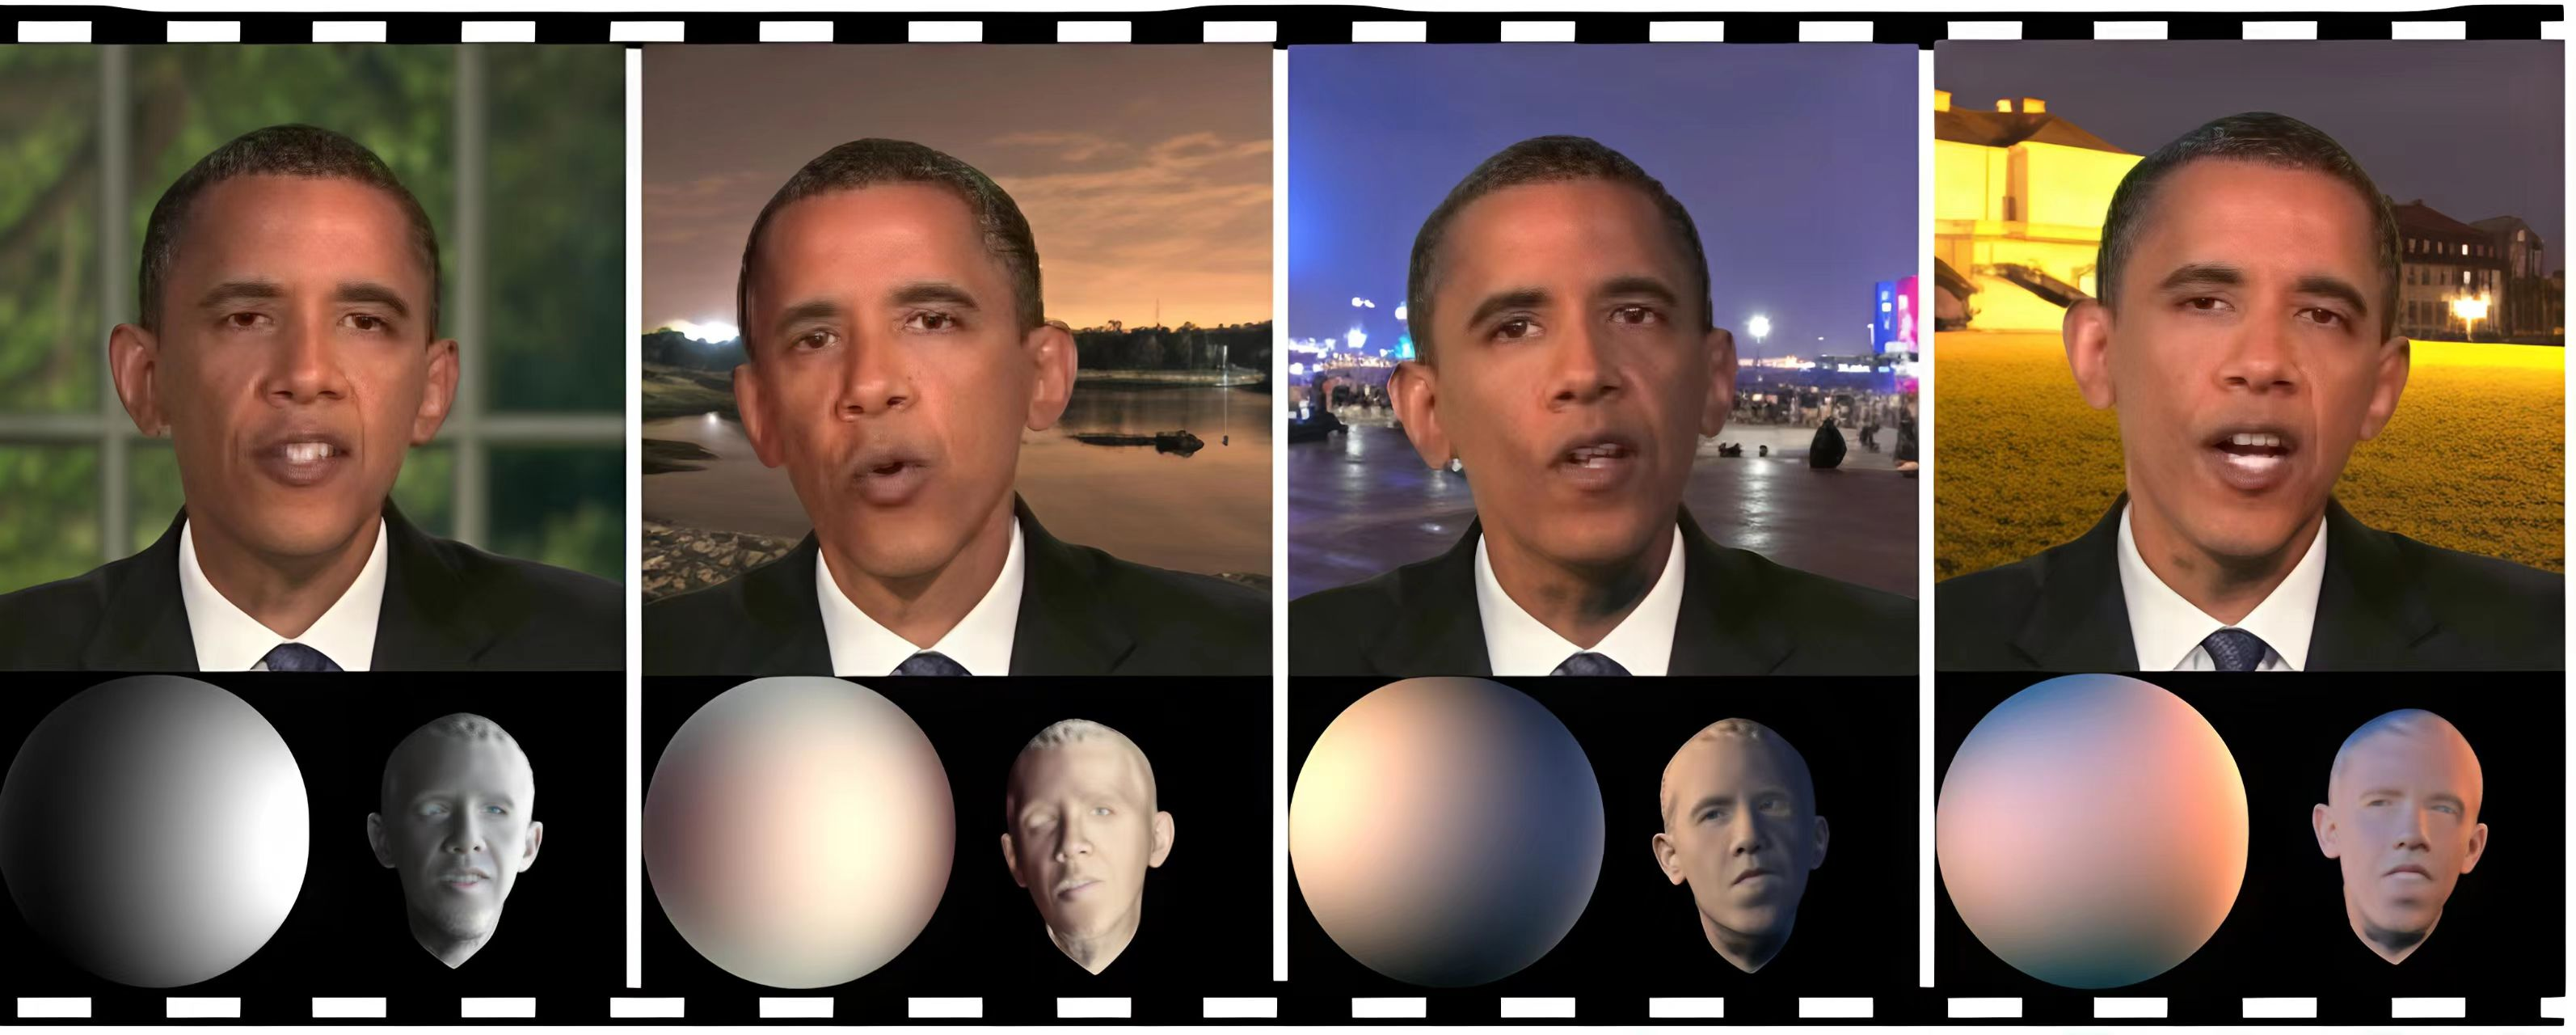
\includegraphics[width=0.7\textwidth,height=4cm]{resources/1p/1-5.jpg}
  % \bicaption{中文标题}{English Caption} % 使用中英文标题
  \caption{人脸视频重光照} % 只使用中文标题
  \label{fig:1-4}
  %\vspace{1 cm} % 使用该指令调整上下间距
\end{figure}
基于静态三维光场人像光照编辑的直接动态扩展，如图\ref{fig:1-4}所示，本质上是直接将单帧图像应用于视频序列，Chan\cite{Chan2022}通过估计人像的表面法线、反射特性与原始光照分布，再利用物理或学习模型在新的光照条件下重建图像，实现光源方向、强度或颜色的改变，从而生成具有目标光照效果的人像。Wang\cite{Ranjan2023}先由抠图模块从单张 RGB 图中提取前景；再经几何网、反照率网分别预测表面法向量与反照率，结合预过滤的漫反射和镜面光图构建像素对齐光照表示；最后由着色网合成含非朗伯效应的重光照结果，进行人像背景的重光照。Zhou\cite{Zhou2019}通过比率图像算法生成 DPR 数据集，用 3DDFA 估算法向量并经 ARAP 扭曲优化，结合 SfSNet 估计的球谐光照。再训练沙漏网络，以源图像和目标光照为输入，采用跳层训练策略，结合多损失函数正则化，最终生成 1024×1024 高分辨率重光照图像。Jiang提出的Nerflighting\cite{Jiang2023}框架，基于 EG3D 构建分离的几何外观潜空间与光照潜空间，通过光照映射网络将球谐系数转化为光照潜码，生成阴影三平面。结合正则化减少分解歧义、提升泛化性，经编码器投影真实人像至潜空间，实现动态光照编辑。Pan提出的ShadeGAN\cite{Pan2021}模型，模型显式解耦了反照率与3D形状。它利用表面法向结合输入的光照参数，通过朗伯着色模型计算像素颜色。仅改变输入的光照条件，即可实现静态人像重光照。然而，是上述方法为静态人像场景设计的，直接应用于视频时，会因为时序一致性差而产生帧间闪烁或和视频播放不自然的显示效果，难以满足三维光场视频显示中对平滑、逼真过渡的需求，并未对三维光场中特有的多视角一致性进行优化。

多视图人像视频同时编辑方法，其本质是对单目人像视频进行光照编辑，先获取到不同视角下的人像视频序列，然后依次使用相同的光照条件进行重光照，最后生成合成视频序列在三维光场上展示。基于Qiu\cite{Qiu2024}提出的提出 ReliTalk 框架，以单目视频为输入，借 FLAME 模型获初始面部几何与法向量，结合语音特征优化法向量图；动态估视频光照，分解反射率为法向量、反照率等；用身份一致性损失优化 3D 表示，最终实现单目人像视频重光照。Zhang提出的基于一致性建模的实时神经人像视频重光照\cite{Zhang2021b}以单目 RGB 视频为输入，构建含 60 余万帧的动态 OLAT 数据集，通过结构与光照解耦、时间建模及光照采样，联合保证语义等一致性，实现动态视频重光照。Wang提出Comprehensive Relighting\cite{Wang2025}框架，针对单目人体视频，依托预训练扩散模型构建粗到细框架，联合建模重光照与背景协调，引入无监督时序光照模型及时空特征融合、引导细化，实现多光照控制下连贯且泛化性强的人像视频重光照。Chandran提出首个端到端可微分的人像视频重光照\cite{Chandran2022}方法，针对单目人像视频逐帧重光照易产生闪烁的问题，联合优化目标光照与时间一致性。无需光照标注，利用现有人像视频训练，通过光照估计损失、时间损失和感知损失约束，结合面部对齐、重光照、合成与一致性网络，生成光照准确且时序连贯的人像视频重光照结果。上述方法是对视频人像进行光照编辑，可以保证较高的时序一致性，但是三维光场视频内容由多视图视频构成，不同视图间的光照信息相互关联，当单独对某一视角的视频序列进行光照编辑时，会使多视图之间的一致性得不到保证,进而削弱三维光场视频人像的真实感与连贯性。

密集视点人像视频现场采集方法如图\ref{fig:1-7}所示，是通过搭建自定义动态光照条件的密集视点采集设备，现场拍摄多视点的带动态光照的人像视频。ReN Human\cite{Xie2024}搭建约三十台同步相机与上百个可控光源组成的球形拍摄系统，通过逐光源点亮方式采集多视角、多光照条件下的人像视频。谷歌提出的The Relightables\cite{Guo2019}系统通过搭建一个包含 336 台高帧率相机与约 5000个可独立控制的 LED 光源的半球形穹顶拍摄装置，实现在多视角和多光照条件下的同步捕获。每一帧图像都对应一个精确记录的光照状态，所有视点同步记录，从而生成带有已知光照条件的多视角人像视频序列。Virtually Being\cite{Xu2025}使用约 75 台同步高分辨率相机 环绕搭建成多视角捕获阵列，并在外部配置 环形可编程 LED 光照系统。在采集过程中，系统通过时间复用光照控制依次激活不同方向与强度的光源，同时所有相机以毫秒级同步拍摄，从多个视角同时记录演员在不同光照条件下的反射与阴影变化。由此获得的包含光照变化信息的多视角视频序列。上述的密集视点人像视频现场采集方法可以得到更高时序一致性和多视角一致性的人像视频序列。但是需要搭建大规模采集设备和光源阵列，对于场地和时间的要求极高。

\begin{figure}[htbp]
  \centering
  % 第一张子图（左侧）
  \begin{minipage}{0.48\textwidth}  % 宽度减半，为左右排列留出空间
    \centering
    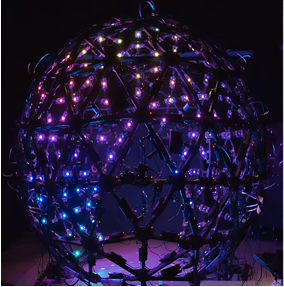
\includegraphics[width=0.9\linewidth, height=7cm]{resources/1p/1-7a.png}
    
    \centering\small(a) 
    \label{fig:1-2a}
  \end{minipage}
  \hfill  % 关键：添加水平间距，让两张图左右分开
  % 第二张子图（右侧）
  \begin{minipage}{0.48\textwidth}
    \centering
    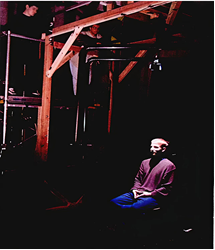
\includegraphics[width=0.9\linewidth, height=7cm]{resources/1p/1-7b.png}
    
    \centering\small(b) 
    \label{fig:1-7b}
  \end{minipage}

  % 大图标题：保持不变
  \caption{ (a) Relightables (b) lightstage}
  \label{fig:1-7}
\end{figure}
\section{论文的组织结构}
本文围绕面向三维光场人像光照编辑这一核心研究课题，立足三维光场显示的工程需求与技术痛点，遵循 “理论奠基 — 静态方法构建 — 动态优化升级 — 实验验证” 的学术逻辑，构建了层次清晰、逻辑闭环的研究框架。全文共分为六章，从基础理论、核心方法到实验验证逐步推进，形成完整的技术体系与学术论证链条，具体组织结构安排如下：

第一章题目是绪论。作为整篇论文的开篇，本章旨在明确研究背景、意义与核心目标，为后续研究奠定整体框架。首先，从三维显示技术的发展趋势切入，阐述裸眼 3D 光场显示的应用价值与市场需求，点明光照编辑在三维光场人像显示中的核心地位 —— 无论是静态场景下的立体结构塑造，还是动态场景下的沉浸感维持，光照均是决定真实感的关键因素。随后，系统梳理国内外研究现状，分别针对三维光场静态人像光照编辑与动态人像视频光照编辑两大方向，分析现有方法的优势与不足，针对当前研究中存在的 “采集设备复杂昂贵”“多视角光照一致性不足”“动态场景时序闪烁” 等核心问题，确立本文的研究切入点。在此基础上，界定研究范围与核心目标，提出具体研究内容：静态三维光场人像光照编辑基础方法、动态场景下时间和空间双维一致性优化策略。最后，给出全文章节组织结构，清晰呈现各部分的逻辑关联。

第二章题目是三维光场人脸光照编辑技术基础。本章是全文的理论基础，为后续方法设计提供科学依据与技术支撑。首先，从人类立体视觉的生理与认知机制出发，解析纹理梯度、透视关系、双目视差等核心深度线索，阐明三维光场显示的生物学原理；随后，详细讲解光场的数学定义与工程化模型，重点分析七维全光函数到四维双平面光场模型的降维逻辑，以及基于光栅的光场显示系统的结构、工作机制与关键参数计算方法。其次，深入阐述三维人像渲染的三大核心物理模型：相机投影模型、球谐函数光照模型（数学推导、展开方式及物理意义）、渲染模型（传统 PBR 渲染与 NeRF 体渲染的原理、优势与局限性）。最后，构建多维度客观评价指标体系，涵盖感知质量（FID、PSNR、SSIM、LPIPS）、WE、LE、LI等大类指标，明确各指标的计算方式与评价标准，为实验验证提供统一的量化依据。

第三章题目是三维光场人像静态光照编辑基础方法。本章作为核心方法的第一阶段，聚焦静态三维光场人像的光照编辑问题。首先，分析静态光场人像光照编辑的痛点：多视图独立编辑导致光照一致性差，密集采集设备成本高昂，因此提出 “关键信息驱动” 的核心思路 —— 通过提取光照关键信息（球面调和系数），在统一框架下实现多视角光照协同编辑。其次，设计完整的静态光照编辑框架，包含三大核心模块：高光去除模块、光照编辑模块、密集视点生成模块。最后，通过系统实验验证方法有效性：客观实验与 NVPR、LRPI 等主流方法对比，在 FID、PSNR 等指标上取得更优结果；主观实验基于三维光场显示器，通过 20 名参与者对 24 组场景的评估，证明方法在立体感（得票率 89.19\%）与光照一致性（得票率 92.29\%）上显著优于单视图依次编辑方法。本章为后续动态场景优化奠定了技术基础。

第四章题目是第四章 三维光场人脸视频动态光照编辑。本章作为核心方法的升级阶段，针对静态方法扩展至视频序列时出现的 “时序闪烁” 与 “多视角光照失配” 等问题，提出时间 - 空间双维联合优化框架。首先，时间维度上，逐帧编辑导致光照跳变；空间维度上，多视角独立优化破坏光照物理一致性。因此，构建两大核心优化模块：时序一致性优化模块（基于特征分离策略，通过共享编码器提取稳定语义特征，光流估计网络实现跨帧空间对齐，光照特征提取网络解耦几何与光照，双重损失函数约束光照时序连续）、多视角一致性优化模块（基于三维几何对齐，通过三维模型表面采样将多视角光照约束转化为三维点光照观测问题，多因子加权聚合获得统一光照值，一致性回投影优化还原至二维视角并保留细节）。最后，通过全面实验验证框架有效性：定量实验与 PTI、SMFR 等方法对比，在时序一致性与多视角一致性指标上的对比，以及时序一致性的消融实验验证模块的必要性，完整模型在所有指标上表现最佳；视觉效果展示证明方法在保留表情动态与细节纹理的同时，有效抑制了光照闪烁与视角偏移。

第五章题目是总结与展望。本章对全文研究工作进行系统性梳理与升华。首先，总结核心研究成果：提出了关键信息驱动的静态三维光场人像光照编辑方法，解决了设备复杂与光照不一致的问题；构建了时间 - 空间双维联合优化框架，突破了动态视频光照编辑的时序与多视角一致性瓶颈。客观分析研究局限性：目前仅适用于人像场景，对复杂非人像场景的适应性不足，实时性有待提升，难以满足高速动态视频的编辑需求。最后，展望未来研究方向：拓展多场景通用性，研究非人像场景的几何与光照解耦方法；优化实时推理性能，通过模型轻量化、硬件加速等方式提升处理速度；融合生成式 AI 技术，实现更精细的光照细节编辑与场景交互；探索多模态输入（文本、语音、草图）的光照编辑方式，进一步降低用户操作门槛。






